\chapter{Methods}
\label{methods}
The James Webb Space Telescope is set to launch some time in 2021, with a
 cost of over \$8.7 billion in the first five years after launch. We need to be
 able to accurately predict how it will operate before it
 launches in order to effectively allocate observation time.
 The Planetary Spectrum Generator (PSG) created by \citet{psgpaper}, was
 designed specifically with this in
 mind, and can simulate a variety of planetary observations using a variety of
 telescopes. The PSG's most important feature is its line-by-line radiative
 transfer model (PUMAS), which depends strongly on the given atmosphere profile.
 The climate models discussed in chapter \ref{models} provide a useful input to
 the PSG, but because the climate models are complex, they must first be
 adapted
 into formats supported by the PSG. The bulk of the work for this thesis was to
 create a data pipeline to make climate models compatible with the PSG. In
 this chapter we will discuss the techniques used to convert the models from
 \citet{wolf17, wolf18} into inputs for the PSG and how the PSG uses those
 inputs to produce spectra.

Climate models have many outputs. Attributes such as temperature, species abundance,
 pressure, and others are stored in latitude by longitude by altitude arrays.
 Other parameters such as surface temperature, albedo, and surface pressure are
 stored in latitude by longitude arrays. Other parameters have only one
 planet-wide value like gravity and orbital period. The output of climate models
 are a
 complex file type that stores all these values, but only a few of them are
 relevant for the PSG. Additionally, some values are not included in the climate
 model such as the distance between the star and the observer, the orbital
 inclination, and others. These parameters are astrophysically important, and
 are therefore needed by the PSG, but are not provided by the climate model
 because they are not atmospherically important, so they must be found elsewhere.

Additional parameters that were not given by the climate model were found using
 NASA's exoplanet archive. The parameters used from the exoplanet archive were
 name, mass, radius, diameter, semi-major axis, inclination, transit depth,
 insolation, star radius, star velocity, star effective temperature, star
 distance,  star magnitude, star metallicity, and star logarithmic surface
 gravity, and are specific to TRAPPIST-1 e.

The PSG only uses an atmospheric profile, so the 3D climate model
 data had to be reduced to a 1D atmospheric profile. How this
 should be done depends on the observational conditions. For an exoplanet
 transit, the significant part of the atmosphere is the
 terminator profile because that is where light from the star will pass through
 the atmosphere and towards the observer. For all other phases, the most
 significant part of the atmosphere is the Earth facing side.

For a transit the phase is $\SI{180}{\degree}$, which means the left hand
 side has a phase of $\SI{270}{\degree}$ and the right hand side has a phase of
 $\SI{90}{\degree}$. For the models in \citet{wolf18}, these phases
 correspond to exactly a single grid cell, but in order to generalize the
 procedure, the average of all cells that fit the criteria of
 $\lambda=\SI{270}{\degree}\pm\SI{5}{\degree} \,\mathrm{\bf{or}}\,
 \lambda=\SI{90}{\degree}\pm\SI{5}{\degree}$ is used. This method would work even if
 there was no longitude corresponding exactly to
 $\lambda=\SI{270}{\degree} \,\mathrm{\bf{or}}\, \lambda=\SI{90}{\degree}$.

For a transit, all longitudes and latitudes are weighted equally because the
 grid cells are spaced evenly across latitudes. In order to compute a transit
 profile, the points are averaged with equal weighting according to the equation

\begin{equation}
    x_i\left(\phi\right)=
    \ddfrac{
        \int_{\SIlist{85;265}{\degree}}^{\SIlist{95;275}{\degree}}
        \int_{\SI{-90}{\degree}}^{\SI{90}{\degree}}
        x_{i,\delta,\lambda}
        \,\dif \delta\dif \lambda
    }
        {\int_{\SIlist{85;265}{\degree}}^{\SIlist{95;275}{\degree}}
        \int_{\SI{-90}{\degree}}^{\SI{90}{\degree}}
        \,\dif \delta \dif \lambda
    },
    \label{transitavgeqn}
\end{equation}
where x is a parameter at a grid cell of height $i$, latitude $\delta$, and
 longitude $\lambda$. Latitude and longitude are averaged, but the heights are
 not, so Equation \ref{transitavgeqn} would reduce a 3D climate model to a 1
 dimensional profile for each parameter x. The parameter x can be used to
 represent temperature, pressure, or volume mixing ratio of any of the tracked
 species.

For the non-transits, many of the variables that were fixed in the transit case are
 no longer constant. To create a non-transiting atmosphere profile, the longitude
 (implicitly as a function of phase) is now a variable. In transits, all grid
 point are equally significant to the atmosphere profile, but for a non-transiting
 profile, some points are more significant than others. Inherent to a
 latitude-longitude grid is the convergence of
 points near the poles. The result is that each grid cell occupies less area
 near the poles, and should therefore be weighted less in the average by a
 factor of $\cos(\delta)$. In addition, the Earth facing side contributes more
 to the emission towards Earth than the limbs. The result of this is a second
 factor of $\cos(\delta)$ to account for the latitudinal component and a factor
 of $\cos(\lambda+\phi)$ to account for the longitudinal component. The
 resulting value is a disk average given by the equation

\begin{equation}
    \mathrm{x}_i\left(\phi\right)=
    \ddfrac{
        \int_{-\phi-\SI{90}{\degree}}^{-\phi+\SI{90}{\degree}}
        \int_{\SI{-90}{\degree}}^{\SI{90}{\degree}}
        \cos^2(\delta)\cos(\lambda+\phi)\mathrm{x}_{i,\delta,\lambda}(\phi)
        \,\dif \delta\dif \lambda
    }
        {\int_{\SI{0}{\degree}}^{\SI{360}{\degree}}
        \int_{\SI{-90}{\degree}}^{\SI{90}{\degree}}
        \cos^2(\delta)\cos(\lambda+\phi)
        \,\dif \delta\dif \lambda
    },
\end{equation}
which is the same as Equation \ref{transitavgeqn}, except for the addition of a
 weighting in the cosine of $\lambda$ and $\delta$, and a dependence on $\phi$.
 Physically, this equation can be described as taking a 3D sphere of the planet
 and simplifying it to a 2D projection as seen by the observer, then averaging
 the observed value \citep{cowanagol08, kollabbot15}. This method means that any
 atmospheric parameter x that varies with respect to $\phi$ should change
 relative to the observer. The cosine squared for latitude indicates that there
 is a strong preference for latitude, and atmospheric features that are
 significantly north or south of the equator should only weakly contribute to
 the disk averaged value.

This disk weighted average explicitly shows the weighting function used, but
implicitly in the integrals, there is also a mask, where only half of the planet
is used in the calculation at any given time. This is because only half of the
planet is facing Earth, and the other half therefore shouldn't contribute to the
average. If the limits were to include the anti-Earth facing side, it would
include negative values due to the cosine term, which would be nonsensical. In
Figure \ref{maskweight}, these two behaviors are shown side by side.

\begin{figure}[ht]
    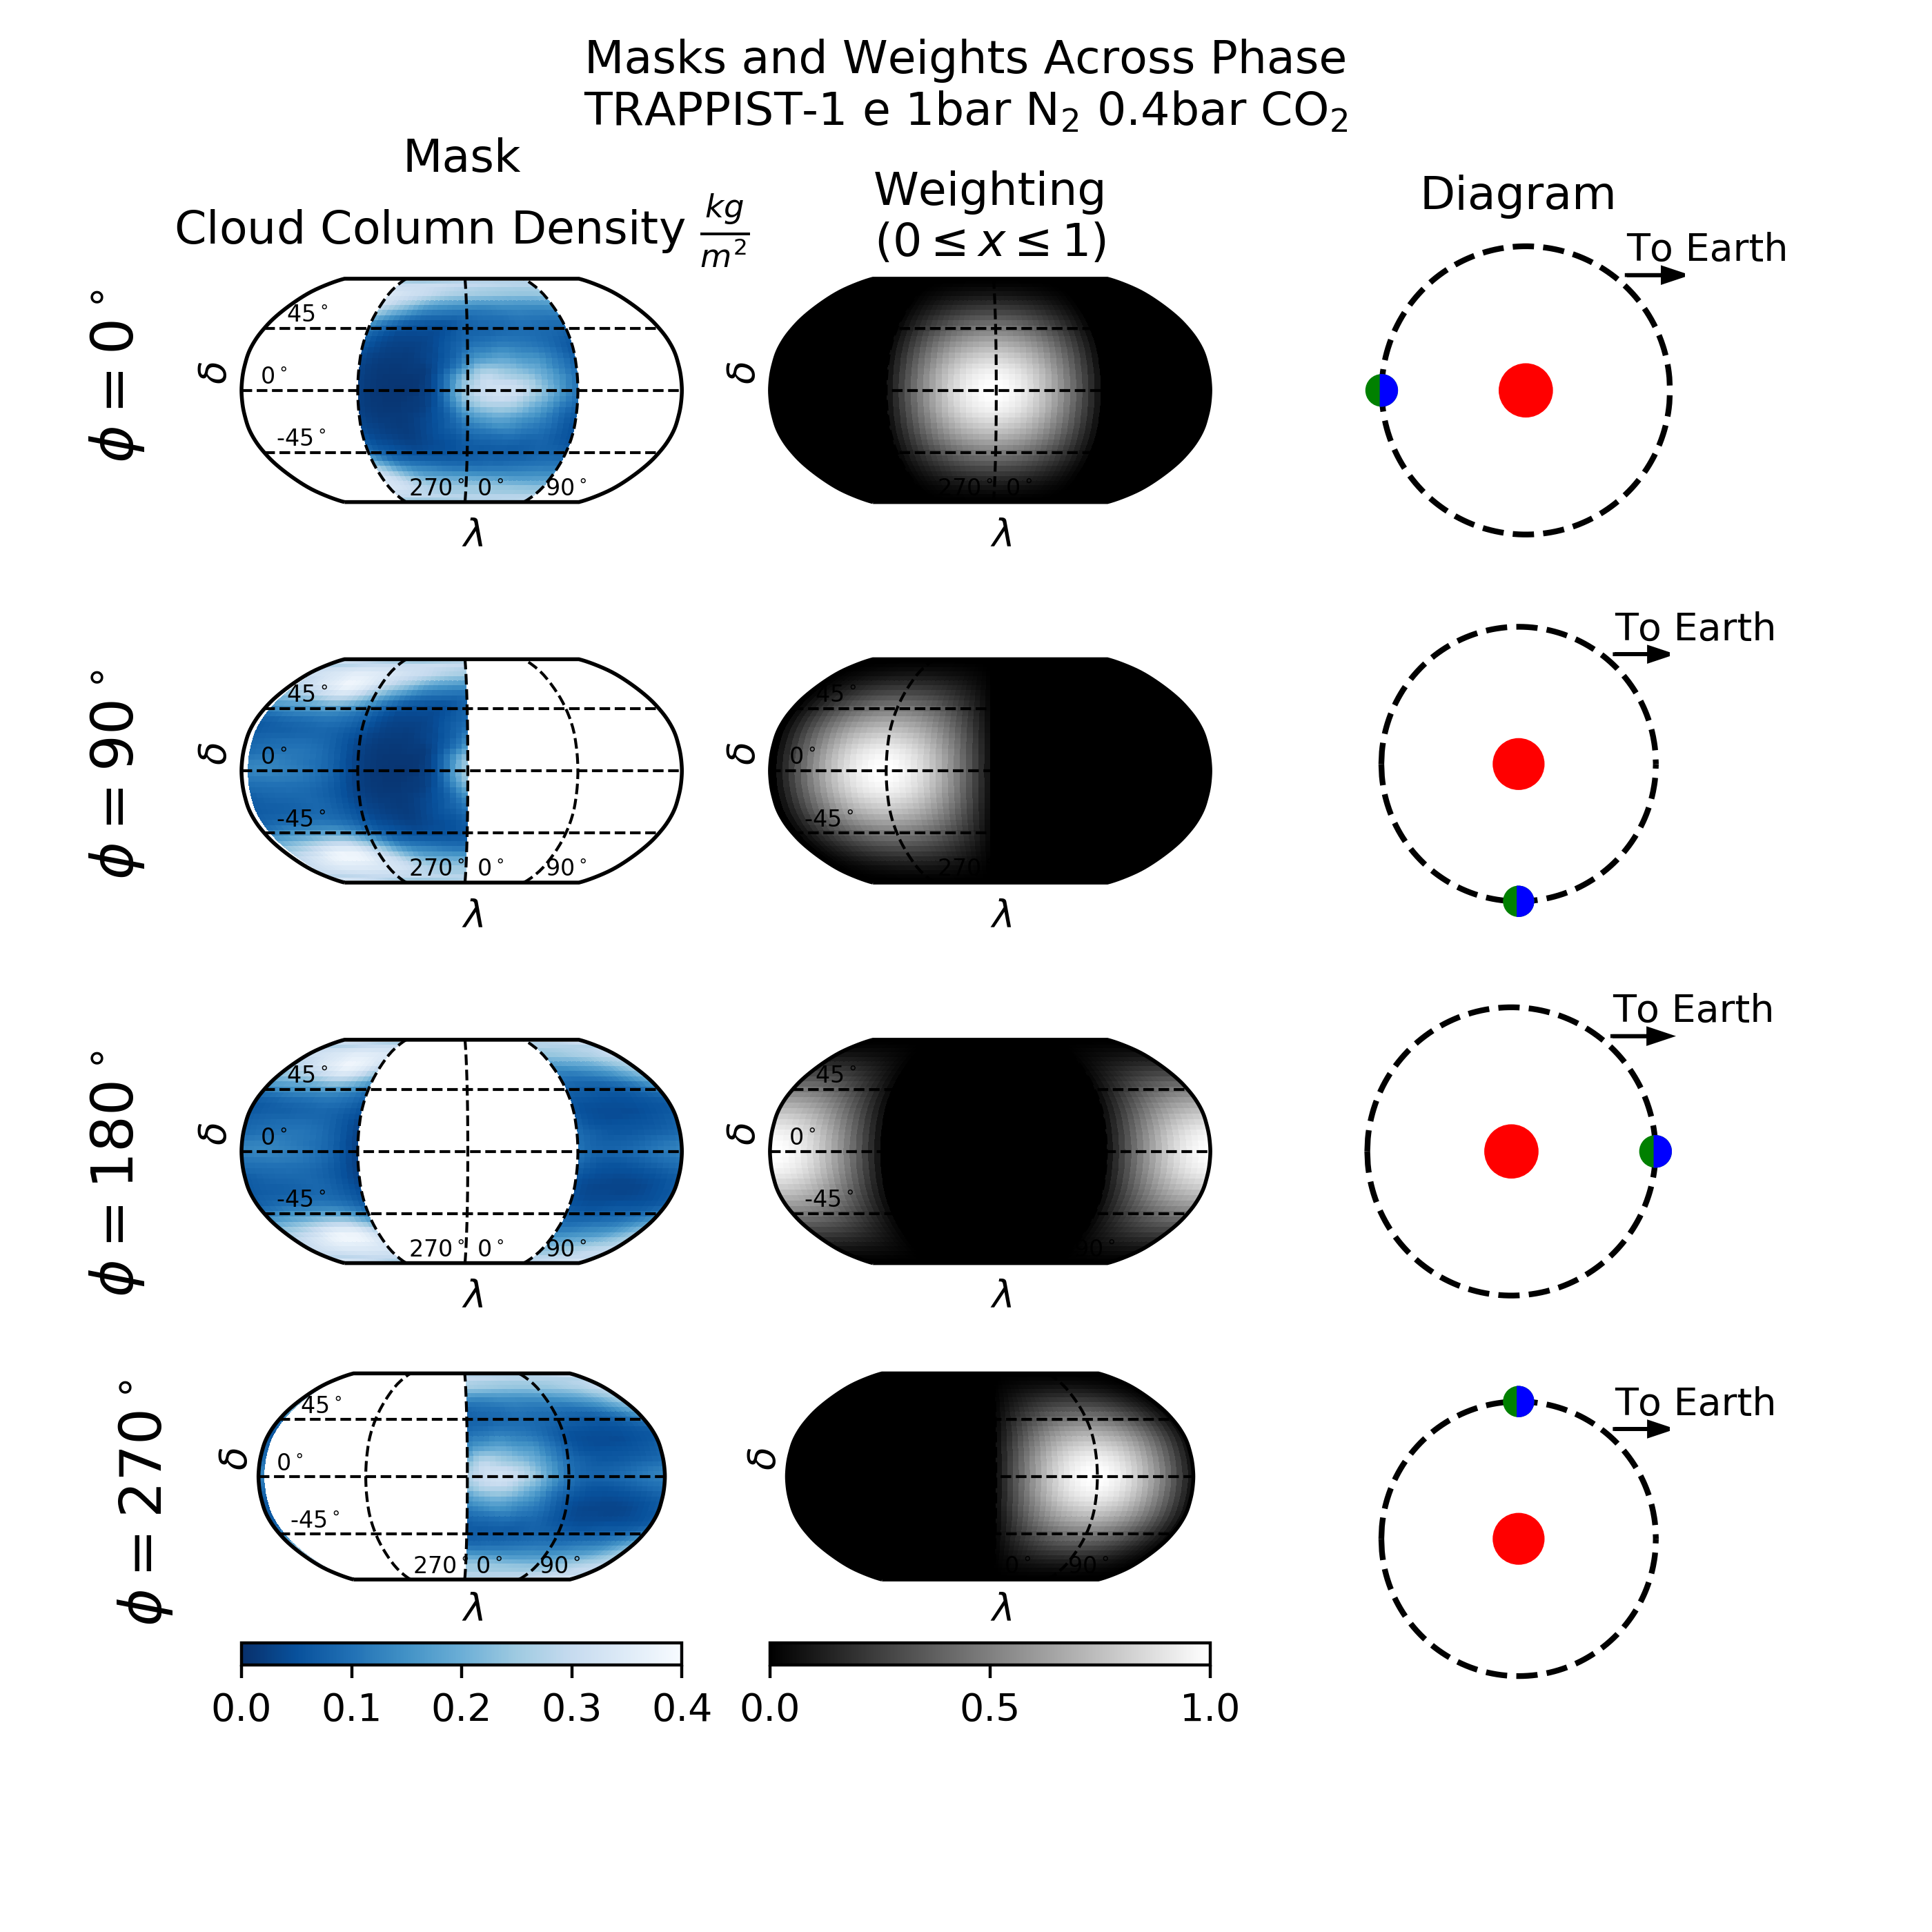
\includegraphics[width=\textwidth]{methods/phases_weights.png}
    \caption[Surface Masks and Weights Across Phases]{Surface masks and weights
    across phase. As a planet rotates through $phi$, the Earth facing side of
    the planet will change. The climate model used in the mask diagram is the
    TRAPPIST-1 e $\SI{1}{\bar}$ \chem{N_2} $\SI{0.4}{\bar}$ \chem{CO_2} case.
    At different points
    through the year, the substellar cloud will move in and out of view.
    Parameters like emissivity should decrease as the cloud is in view and
    increase when the western side without clouds are in view.}
    \label{maskweight}
\end{figure}

For transits, a different masking scheme is used, and no weighting
 scheme is used. A similar diagram to Figure \ref{maskweight} is given for the
 transit case in Figure \ref{transitweight}.

\begin{figure}[ht]
    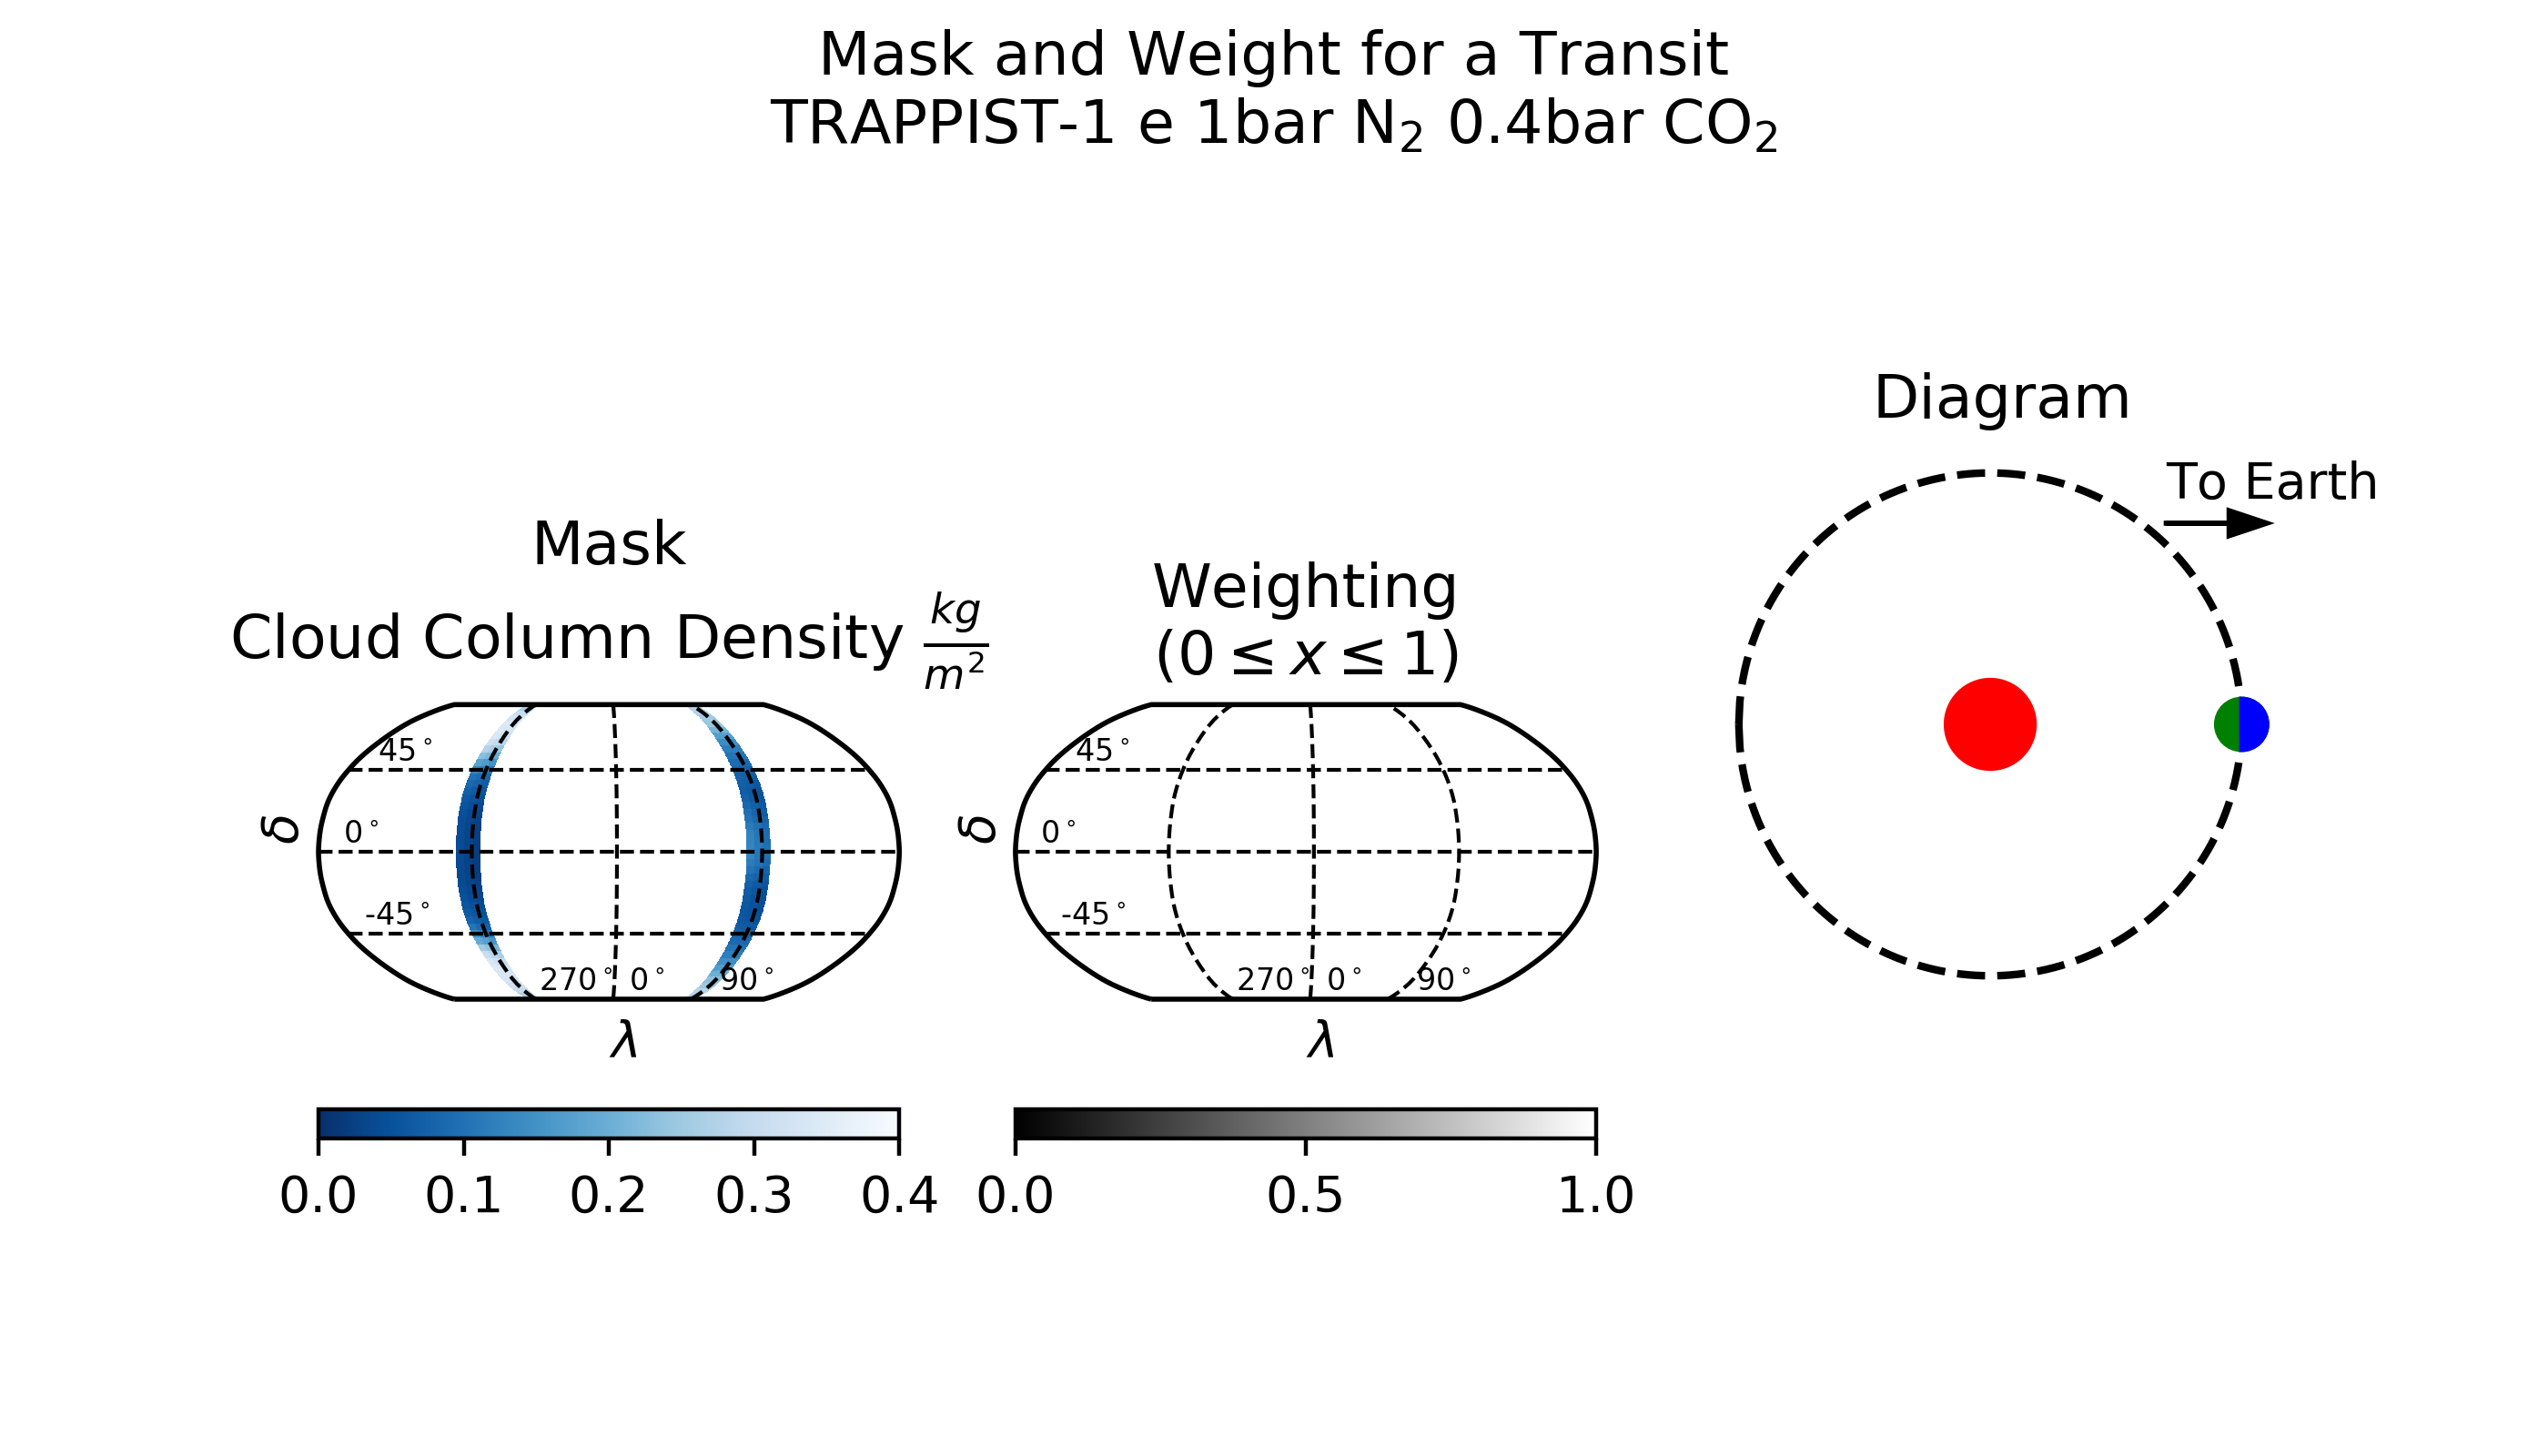
\includegraphics[width=\textwidth]{methods/transit_weights.png}
    \caption[Surface Mask and Weights for Transits]{Surface masks and weights
    for transits. For the transiting case, a weighting function is unnecessary,
    but it is included for consistency with Figure \ref{maskweight}. The more
    significant detail is that the masking scheme is discontinuous with the disk
    averaged values over the remainder of the exoplanet's year.}
    \label{transitweight}
\end{figure}

The whole purpose of averaging these values is that the 3D climate model can be
 reduced to an atmosphere profile that can be put into the PSG. The parameters
 used from the climate model profile were height, pressure, temperature, and the
 volume mixing ratios of \chem{N_2}, \chem{CO_2}, \chem{CH_4}, \chem{H_2O},
 liquid clouds, ice clouds, liquid cloud size, ice cloud size. Additionally,
 surface pressure, surface temperature, surface albedo, and dry molecular weight
 were used, but they do not vary with height, so they are not part of the
 profile, although they are still taken by the PSG as a separate parameter.

In an exoplanet transit, light passes through the atmosphere and is collected
 by a telescope. A majority of an exoplanet's atmosphere is far too thick for
 light to enter one side and exit the other. As light passes through any
 medium that could absorb it, it should be extinguished according to Beer's Law

\begin{equation}
    \frac{I}{\mathrm{I_0}}=\exp(-n \sigma L),
\end{equation}
where $I$ is the intensity of the light as seen by the observer, $\mathrm{I_0}$
 is the intensity of the light at the source, $n$ is the particle number
 density, $\sigma$ is the cross-sectional area of the particles, and $L$ is the
 length of the path that light travels. In an exoplanet transit at low
 altitudes, $n$ is far too large, so $\nicefrac{I}{\mathrm{I_0}}$ is too small to
 be detected. While $\sigma$ won't vary much across an atmosphere, $n$ and $L$
 will decrease as a function of height. $n$ will decrease
 exponentially as given by the equation

\begin{multicols}{2}
    \begin{equation}
    \frac{n}{\mathrm{n_0}}=\exp\left(-\frac{z}{\mathrm{H}}\right)
    \end{equation}
    \break
    \begin{equation}
    H=\frac{\mathrm{k_B}T}{\mathrm{mg}},
    \end{equation}
\end{multicols}
\noindent
where $z$ is the height, $n$ is the volume density, $\mathrm{k_B}$ is the
 Boltzmann constant, $T$ is the atmospheric temperature, m is the average
 molecular weight, and g is the gravitational force. This means the upper
 atmosphere will be much less dense than the lower atmosphere. The CAM4 climate
 models only have grid points down to $\SI{1}{\milli\bar}$. Pressures below
 $\SI{1}{\milli\bar}$ are not considered as they are not significant for
 atmospheric dynamics. However, for transit spectra, $\SI{1}{\milli\bar}$ is
 still relatively opaque, and $n$ must be decreased even more for significant
 amounts of light to pass through the atmosphere. To amend the atmosphere models
 for the purposes of transit spectra, additional layers must be added to the
 atmosphere, and these layers must also have pressure drop off exponentially.
 While temperature decreases with height for most of the atmosphere, this
 effect is ignored,
 and all the added layers have a constant temperature given by the top layer of
 the climate model. Additionally, the ratios of all atmospheric species are kept
 the same as the top layer of the climate model.

For the purposes of the PSG, only a few layers were added because the PUMAS
 radiative transfer model includes a very accurate sub-layering scheme. For all
 simulations used in this project, 7 layers were added, and the top layer was at
 a pressure of $\SI{10d-6}{\milli\bar}$. Pressures this low are well beyond the
 necessary range and guarantee that the PSG will have atmospheric inputs capable
 of simulating an exoplanet transit.

The PSG can produce a variety of outputs, the most fundamental of which are
 $\si{\watt.\meter^{-2}.\steradian^{-1}.\micro\meter^{-1}}$ and ADU, which
 represent what a
 telescope would actually see. The PSG can also return an already reduced output
 that simply shows the transit depth. This reduced method can be derived from
 either raw method, but is more convenient for analysis, and is therefore the
 most commonly used. The PSG can produce a spectra, as well as a breakdown of
 its components by sources, although it's worth noting that none of those
 components can actually be observed in an exoplanetary system. In an actual
 exoplanet observation, only the raw total signal can be observed.

The results from the PSG separate the noise from the signal, although that's not
 how it would actually be observed. Signals without noise allow us to make
 predictions about observations, and noise can be used later to determine how
 long it would take to make conclusions about those observations. There are
 other noise simulators for JWST that rival that of the PSG, and often
 could use the PSG's spectra as an input. For this reason, the PSG only needs
 to be run once to get results on the signal, and the exposure time doesn't
 impact those results. Exposure time would only affect the signal-to-noise
 ratio.

For transits, the PSG needs to be run only once using the terminator mean
 profile. For thermal phase curves, the thermal emitted flux must be computed at
 each point of the planet's orbit, so the PSG must be run multiple times to
 compute a thermal phase curve. Thermal phase curves should vary continuously,
 and so one might assume that they could compute thermal phase curves with
 arbitrary resolution. However, this isn't possible using 3D climate models because
 the averaged atmosphere profile won't change unless $\phi$ varies by more than
 $\SI{5}{\degree}$ because  that is the longitudinal resolution of the climate
 models. In Figure \ref{maskweight}, the individual grid cells of the climate
 model can be seen by eye. The grid cell size defines the limiting temporal
 resolution of a thermal phase curve. This means that in order to compute thermal
 phase curves with higher resolution than $\SI{5}{\degree}$, it would require higher
 resolution climate models. However, the point is moot, TRAPPIST-1 e has an
 orbital period of $\SI{6.01}{\day}$ \citep{trappistdiscovery}, and therefore orbits at a
 rate of $\sim\SI{2.5}{\degree\per\hour}$. In an actual observation of a
 thermal phase curve, it's reasonable to be observing for multiple hours, so a
 climate model with 72 longitudinal bins will have similar or greater resolution
 in $\phi$ than the maximum possible resolution from observations in ideal
 conditions.